\documentclass{standalone}
\usepackage{tikz,color}
\begin{document}


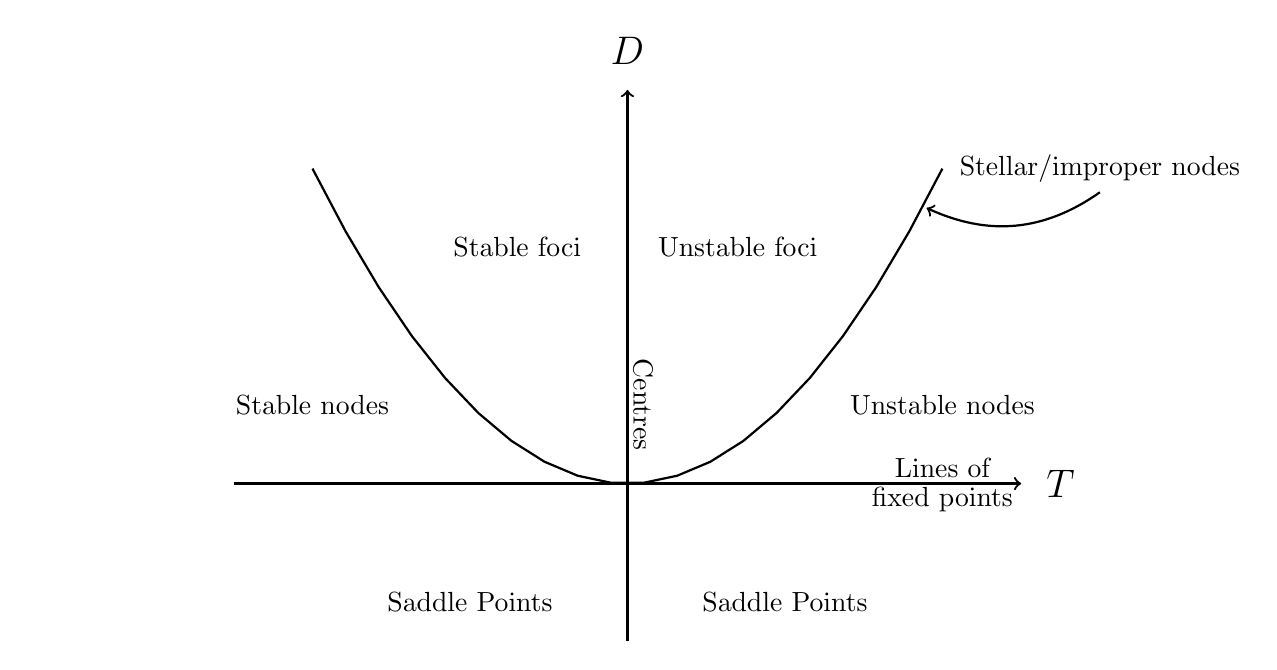
\begin{tikzpicture}
\draw [->,thick] (-5,0) to (5,0);
\draw [->,thick] (0,-2) to (0,5);
\draw [-, thick, domain=-4:4, samples=20] plot({\x },{0.25*\x*\x});
\node at (0,5.5) {\Large{$D$}};
\node at (5.5,0) {\Large{$T$}};
\node at (-4,1) {Stable nodes};
\node at (4,1) {Unstable nodes};
\node at (-1.4,3) {Stable foci};
\node at (1.4,3) {Unstable foci};
\node at (-2,-1.5) {Saddle Points};
\node at (2,-1.5) {Saddle Points};
\node [rotate=-90] at (0.2,1) {Centres};
\node at (6,4) {Stellar/improper nodes};
\node at (-7.5,4) {};
\node at (4,0.2) {Lines of};
\node at (4,-0.2) {fixed points};
\draw[->,thick] (6,3.7)[bend left] to (3.8,3.5);

\end{tikzpicture}

\end{document}
